After the ``congestion collapse" and with the growth in the last few decades of
 \begin{wrapfigure}{l}{0.5\textwidth}
  \begin{center}
    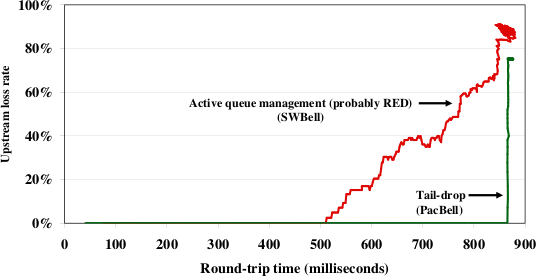
\includegraphics[width=0.48\textwidth]{img/overflows}
  \end{center}
  \caption{How Tail-drop management and RED AQM overflows\cite{Dischinger2007CRB}}
  \label{tdredof}
\end{wrapfigure}

Internet, it has become clear that the TCP congestion avoidance mechanisms,
while necessary and powerful, are not enough to provide a fully safe service,
and the control that can be accomplished from the edges of the networks has
proof that has a limit. So, in order to obtain a good service in all
circumstances, some mechanisms in the routers to complement this endpoint
congestion avoidance mechanisms are needed.\\

Two classes of router algorithms related with congestion avoidance control can
be distinguished: ``queue management" and ``scheduling" algorithms. While the
first one manage the length of packet queues by dropping packets when necessary
or appropriate, the second one determine which packet to send next, and are used
to manage the allocation of bandwidth among flows. It is important to notice
that while this two mechanisms are closely related, the performance that they
address are rather different and should be seen as complementary, and not as
replacements for each other.\\


